% Define custom objects
\tikzstyle{block} = [rectangle, rounded corners, minimum width=3cm, minimum height=1cm, text centered, draw=black, fill=gray!20]
\tikzstyle{arrow} = [thick,->,>=stealth]
\tikzstyle{double_arrow} = [thick,<->,>=stealth]

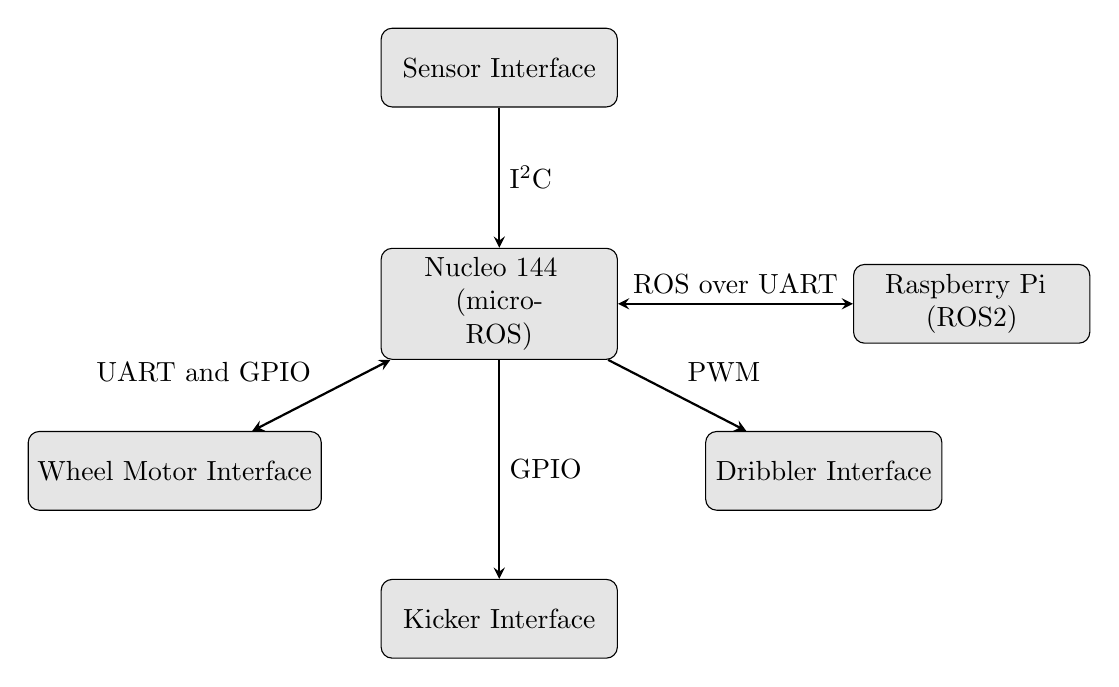
\begin{tikzpicture}[node distance=3cm]

    % Draw nodes
    \node (sensors) [block] {Sensor Interface};
    \node (nucleo) [block, text width=1.9cm, below of=sensors] {Nucleo 144 \newline (micro-ROS)};
    \node (raspberry) [block, text width=2.2cm, right of=nucleo, xshift=3cm] {Raspberry Pi \newline (ROS2)};
    \node (wheel) [block, below left of=nucleo, xshift=-2cm] {Wheel Motor Interface};
    \node (kicker) [block, below of=nucleo, yshift=-1cm] {Kicker Interface};
    \node (dribbler) [block, below right of=nucleo, xshift=2cm] {Dribbler Interface};
    
    % Draw connections
    \draw [arrow] (sensors) -- (nucleo) node[midway, right] {I$^2$C};
    \draw [double_arrow] (nucleo) -- (raspberry) node[midway, above] {ROS over UART};
    \draw [double_arrow] (nucleo) -- (wheel) node [midway, left, yshift=0.3cm] {UART and GPIO};
    \draw [arrow] (nucleo) -- (kicker) node[midway, right] {GPIO};
    \draw [arrow] (nucleo) -- (dribbler) node[midway, right, yshift=0.3cm] {PWM};

\end{tikzpicture}